\entry{2026-10-18}{Priority 3: head latent size $K$ --- the other reading of ``$k$''}

Lane \texttt{2026-10-18-jcp-heads}, last commit \texttt{0ba9a1288}, mirror \texttt{ed3d0c841}. Nine jobs (A100/H200, \texttt{jax\_backend=gpu}), 3.68 of 35 GPU-h, nothing deferred; results audit 3 RESULTS-CONFIRMED, report audit 6 READY. \textbf{Exploratory validation evidence only} (no family-wise claim); errors E0-conditional. Numbers quoted from the generated \path{report.md}.

\begin{itemize}
\item \textbf{Training:} 12 heads ($K\in\{4,8,16,32\}\times$ 3 seeds), the incumbent's exact recipe and data. Oracle error falls from 3.4--7.9\,\% at $K=4$ to 0.29\,\% at $K=32$.
\item \textbf{Qualification is the bottleneck:} at $1024^2$ (BE) only $K=16$ seeds \{0, 1\} and $K=32$ seed \{1\} pass the every-case solver check; $K=4$ and $K=8$ none. So \textbf{error vs $K$ is inconclusive}, and so is the nonlinear-manifold question (F5).
\item \textbf{Head vs linear span:} at matched dimension ($K=r=16$) the head is far more accurate (1.44\,\% vs 10.2\,\% median) but costs 3.78$\times$ more. \textbf{At no more online cost the linear span wins}: $r=128$ reaches 1.10\,\% at 0.59$\times$ the head's cost. Coordinator recheck from per-case values: 1.43\,\%, 1.10\,\%, 10.17\,\%; the $r=128$ value matches priority 1 (1.095\,\%).
\item \textbf{Cost vs mesh:} flat for the $K=16$ head (ratio 1.064) and the incumbent (1.029). Cost vs $K$: no identifiable exponent.
\end{itemize}
\begin{center}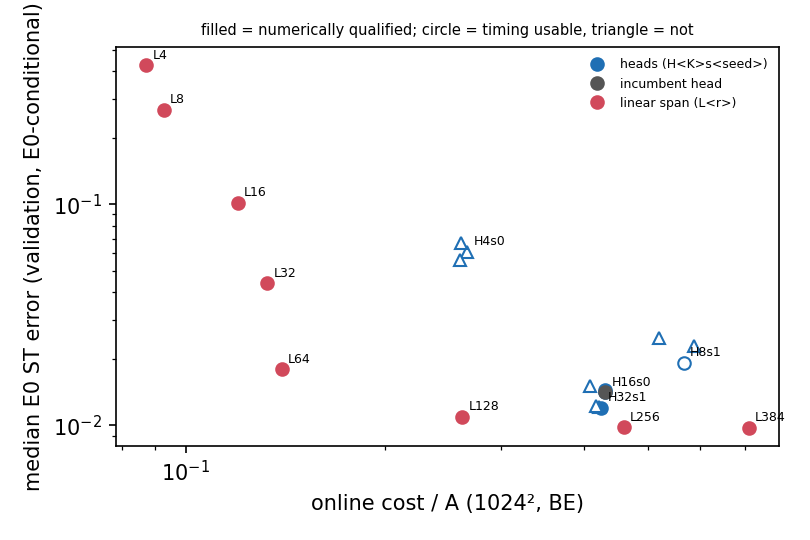
\includegraphics[width=0.48\linewidth]{figs/h_error_cost_1024.png}\hfill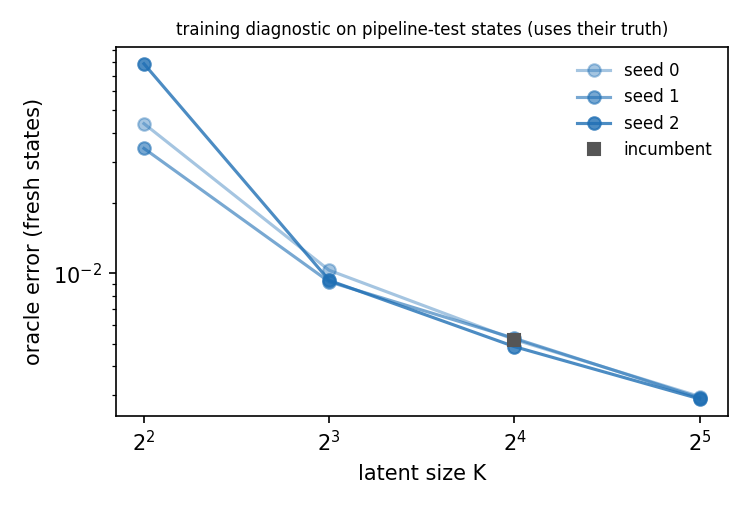
\includegraphics[width=0.48\linewidth]{figs/h_oracle_vs_K.png}\end{center}

\subsection*{Qualified, not retracted}
The 2026-09-14 claim ``the head is necessary at matched latent dimension'' still holds at matched dimension; it does not hold for accuracy per unit cost. The seed-0 $K=16$ retrain equals the incumbent to round-off (same-seed replay, not an independent replication). Head-repair hypotheses (E3c) were not tested.
